\documentclass[12pt]{article}

\author{Pablo Vargas Bermúdez}

\usepackage[margin=3cm]{geometry}
\usepackage{graphicx}
\usepackage{pdfpages}
\usepackage{minted}

\begin{document}
\pagestyle{empty}
\includepdf[pages=-]{Portada1}

\section*{Planteamiento}
Elabora un Programa que pueda leer los nombre de los archivos que
contienen las infecciones por día del Conavid-19, deberá de mostrar la
Lista de los archivos contenidos en el directorio de "infecciones", al
seleccionar un nombre de archivo de la lista, deberá de leer los datos
de ese archivo y cargarlos en un Jtable que muestre toda la
información.

No olvide poner el Jtable dentro de un JScrollPane.

\section*{Código}

\subsection*{Clase Data Builder}
\inputminted{Java}{DataBuilder.java}
\subsection*{Clase Covid}
\inputminted{Java}{Covid.java}
\subsection*{Clase de Prueba}
\inputminted{Java}{Prueba.java}

\section*{Ejecución}
\begin{figure}[ht]
  \centering
  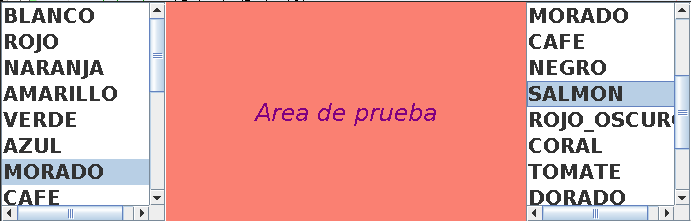
\includegraphics[width=\textwidth]{figures/run1.png}
  \caption{Primera prueba}
\end{figure}
\begin{figure}[ht]
  \centering
  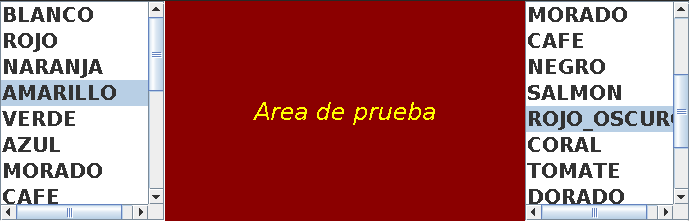
\includegraphics[width=\textwidth]{figures/run2.png}
  \caption{Segunda prueba}
\end{figure}
\begin{figure}[ht]
  \centering
  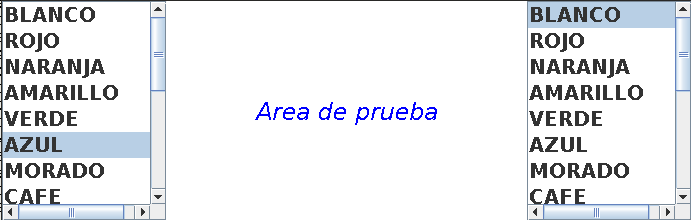
\includegraphics[width=\textwidth]{figures/run3.png}
  \caption{Tercera prueba}
\end{figure}

\end{document}
